\section{Gestion des factures}

\subsection{Objectif du module}

Le module de facturation transforme une consommation validée en facture enregistrée. Il calcule les montants selon les tranches tarifaires, applique la TVA de 18 \%, génère un numéro unique, enregistre la facture et permet sa consultation par le client et le fournisseur.

\subsection{Tarification}

Les tarifs sont stockés dans la table \texttt{tarif}. Chaque ligne contient un type (\texttt{EAU} ou \texttt{ELEC}), une borne minimale, une borne maximale et un prix unitaire. Les tranches sont appliquées de manière progressive.

\begin{table}[H]
\centering
\caption{Tranches tarifaires de l'eau et de l'électricité}
\label{tab:tranches}
\small
\begin{tabular}{p{0.14\textwidth}p{0.22\textwidth}p{0.22\textwidth}p{0.22\textwidth}}
\toprule
\textbf{Type} & \textbf{Tranche 1} & \textbf{Tranche 2} & \textbf{Tranche 3} \\
\midrule
Eau & 0--6 m\textsuperscript{3} : 2,37 DH & 6--20 : 7,39 DH & 20--35 : 10,98 DH ; >35 : 11,03 DH \\
Électricité & 0--100 kWh : 0,82 DH & 100--150 : 0,92 DH & >150 : 1,10 DH \\
\bottomrule
\end{tabular}
\end{table}

Pour chaque tranche, le montant est calculé sur la quantité effectivement consommée dans l'intervalle :

\[
M = \sum_{t} \left( \min(C, borne_{max,t}) - borne_{min,t} \right) \times prix_t
\]

\subsection{TVA et arrondis}

La TVA est fixée à 18 \%. Les montants sont arrondis à deux décimales :

\[
HT = M_{eau} + M_{elec}, \qquad TVA = HT \times 0{,}18, \qquad TTC = HT + TVA
\]

\subsection{Génération de la facture}

La génération est prise en charge par \texttt{Traitement/FactureService.php}. Les étapes sont les suivantes :

\begin{enumerate}[leftmargin=*]
  \item vérifier que la consommation est à l'état \texttt{VALIDEE} ;
  \item vérifier qu'aucune facture n'existe déjà pour cette consommation ;
  \item récupérer le client, le fournisseur, les index et les tarifs ;
  \item calculer les consommations d'eau et d'électricité ;
  \item calculer les montants HT, TVA et TTC ;
  \item générer le numéro \texttt{FAC-YYYYMM-\{id\_conso\}} ;
  \item insérer la facture et passer la consommation à l'état \texttt{FACTUREE} dans une transaction ;
  \item annuler la transaction en cas d'échec.
\end{enumerate}

\begin{lstlisting}[language=PHP,caption={Principe de génération transactionnelle},label={lst:facture}]
$this->pdo->beginTransaction();
try {
    $this->factures->create([...]);
    $this->consommations->changerStatut($idConso, 'FACTUREE');
    $this->pdo->commit();
} catch (Throwable $e) {
    if ($this->pdo->inTransaction()) {
        $this->pdo->rollBack();
    }
    throw $e;
}
\end{lstlisting}

\subsection{Numéro et état de la facture}

Le numéro est unique et construit à partir de la période et de l'identifiant de la consommation. L'état initial est \texttt{IMPAYEE}. Le passage à \texttt{PAYEE} et l'enregistrement d'un paiement sont réservés à une version ultérieure.

\subsection{Consultation et contrôle d'accès}

Le client consulte uniquement ses propres factures. Le fournisseur consulte les factures de ses clients. La liste présente le numéro, la date, la période, les consommations, le montant TTC, l'état et un lien vers le détail.

\begin{figure}[htbp]
  \centering
  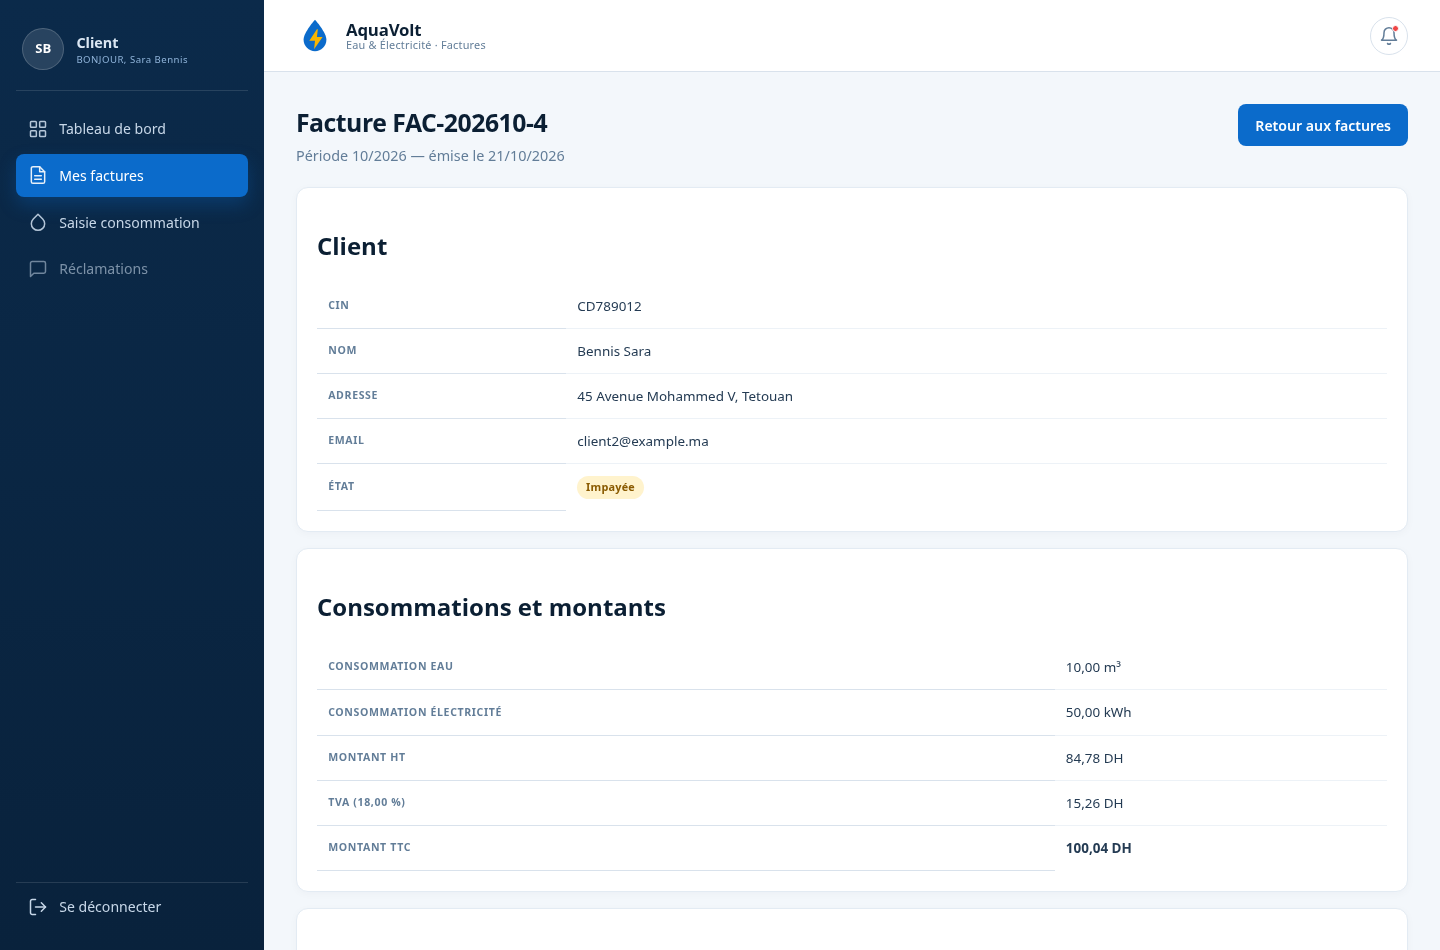
\includegraphics[width=0.72\textwidth]{figures/facture_detail.png}
  \caption{Détail d'une facture avec montants et photos}
  \label{fig:facturedetail}
\end{figure}

\subsection{Exemples de calcul}

\begin{table}[H]
\centering
\caption{Exemples de calculs de facture}
\label{tab:calculs}
\small
\begin{tabular}{p{0.14\textwidth}p{0.14\textwidth}p{0.14\textwidth}p{0.14\textwidth}p{0.14\textwidth}p{0.14\textwidth}}
\toprule
\textbf{Eau} & \textbf{Élec.} & \textbf{HT} & \textbf{TVA} & \textbf{TTC} & \textbf{Cas} \\
\midrule
25 m\textsuperscript{3} & 200 kWh & 355,58 & 64,00 & 419,58 & Référence \\
10 m\textsuperscript{3} & 50 kWh & 84,78 & 15,26 & 100,04 & Saisie valide \\
0 m\textsuperscript{3} & 50 kWh & 41,00 & 7,38 & 48,38 & Correction \\
\bottomrule
\end{tabular}
\end{table}

\subsection{Manuel d'utilisation}

\begin{enumerate}[leftmargin=*]
  \item démarrer le serveur PHP ou Apache et ouvrir l'application ;
  \item se connecter avec un compte client ou fournisseur ;
  \item le fournisseur gère les clients depuis le menu \textit{Clients} ;
  \item le client saisit ses index depuis \textit{Saisie consommation} et téléverse les deux photos ;
  \item en cas d'anomalie, le client confirme ou corrige ;
  \item la facture est générée automatiquement et accessible depuis \textit{Mes factures} ;
  \item le fournisseur consulte toutes les factures depuis le menu \textit{Factures}.
\end{enumerate}

\subsection{Tests du module}

Les tests vérifient la génération après une saisie valide, après confirmation d'une anomalie et après correction, l'unicité de la facture, les montants HT/TVA/TTC, l'accès du client à ses seules factures et l'accès du fournisseur aux factures de ses clients.
